
\documentclass[tikz,border=8pt]{standalone}
\usetikzlibrary{arrows.meta,positioning,fit,backgrounds,calc}
\definecolor{adamw}{HTML}{0072B2}
\definecolor{muon}{HTML}{D55E00}
\definecolor{softblue}{HTML}{E8F1FA}
\definecolor{softorange}{HTML}{FFF1E8}
\definecolor{softgray}{HTML}{F4F4F2}
\begin{document}
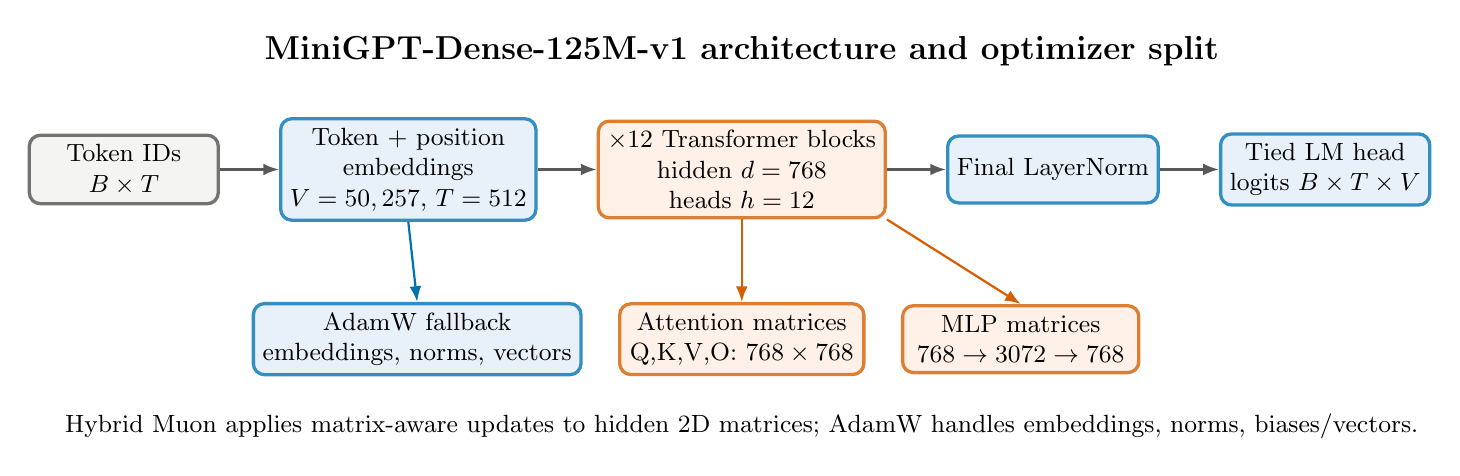
\begin{tikzpicture}[
  box/.style={rounded corners=4pt, draw=black!55, very thick, align=center, minimum height=0.85cm, font=\small},
  arrow/.style={-{Latex[length=2mm]}, thick, draw=black!65},
  muonbox/.style={box, fill=softorange, draw=muon!80},
  adamwbox/.style={box, fill=softblue, draw=adamw!80},
  neutral/.style={box, fill=softgray}
]
\node[neutral, minimum width=2.4cm] (tok) {Token IDs\\$B \times T$};
\node[adamwbox, right=0.75cm of tok, minimum width=2.8cm] (emb) {Token + position\\embeddings\\$V=50,257$, $T=512$};
\node[muonbox, right=0.75cm of emb, minimum width=3.5cm] (blocks) {$\times 12$ Transformer blocks\\hidden $d=768$\\heads $h=12$};
\node[adamwbox, right=0.75cm of blocks, minimum width=2.5cm] (ln) {Final LayerNorm};
\node[adamwbox, right=0.75cm of ln, minimum width=2.6cm] (head) {Tied LM head\\logits $B \times T \times V$};

\draw[arrow] (tok) -- (emb);
\draw[arrow] (emb) -- (blocks);
\draw[arrow] (blocks) -- (ln);
\draw[arrow] (ln) -- (head);

\node[muonbox, below=1.05cm of blocks, minimum width=3.1cm] (attn) {Attention matrices\\Q,K,V,O: $768\times768$};
\node[muonbox, right=0.45cm of attn, minimum width=3.0cm] (mlp) {MLP matrices\\$768\to3072\to768$};
\node[adamwbox, left=0.45cm of attn, minimum width=3.0cm] (fallback) {AdamW fallback\\embeddings, norms, vectors};
\draw[arrow, draw=muon] (blocks.south) -- (attn.north);
\draw[arrow, draw=muon] (blocks.south east) -- (mlp.north);
\draw[arrow, draw=adamw] (emb.south) -- (fallback.north);

\node[font=\bfseries\large, above=0.55cm of blocks] {MiniGPT-Dense-125M-v1 architecture and optimizer split};
\node[align=center, font=\small, below=0.35cm of attn] {Hybrid Muon applies matrix-aware updates to hidden 2D matrices; AdamW handles embeddings, norms, biases/vectors.};
\end{tikzpicture}
\end{document}
